\chapter{Implementacja}
\thispagestyle{firststyle}

\section{Technologia}
    
    Gra została stworzona w formie aplikacji internetowej (webowej).
    Do zalet takiego rozwiązania należy brak konieczności pobrania i instalacji programu na komputerze, niezależność od~platformy oraz większa łatwość utrzymania aplikacji.
    Aplikację zbudowano w oparciu o~stos MEAN (zestaw technologii \emph{open source} bazujących na języku JavaScript, składający się z bazy danych MongoDB, frameworków Express i Angular oraz środowiska Node.js).
    
    Kliencką część aplikacji (\emph{frontend}) wykonano z wykorzystaniem frameworka Angular w~wersji szóstej.
    Serwerowa część aplikacji (\emph{backend}) wykonana została w środowisku Node.js w~wersji ósmej, z użyciem frameworka Express.
    Aplikację umieszczono na platformie chmurowej Heroku.
    Do przechowywania danych wykorzystano nierelacyjną bazę danych MongoDB z zastosowaniem chmurowej usługi MongoDB Atlas.
    
    Grafika gry wykonana została z użyciem programu Inkscape, oprogramowania \emph{open source} do tworzenia grafiki wektorowej.
    Dźwięki nagrano za pomocą mikrofonu Novox NC-1 i~programu \emph{open source} Audacity.
    
    Aplikacja dostępna jest pod adresem \url{https://www.gra-aha.pl}.
    Kod źródłowy umieszczony został w zdalnym repozytorium na platformie GitHub pod adresem \url{https://github.com/Reienn/cogni-thesis}.  
    
\section{Funkcjonalności aplikacji}
    
    \subsection{Rejestracja i logowanie}
        Aplikacja umożliwia rejestrację jako gracz lub jako opiekun.
        W formularzu rejestracji należy podać unikalną nazwę użytkownika, adres e-mail, hasło, powtórzone hasło oraz typ konta.
        W przypadku wyboru konta gracza możliwe jest wprowadzenie loginu opiekuna, który będzie miał dostęp do statystyk i edycji treści gry gracza.
        Po pomyślnej walidacji formularza (formatu adresu e-mail, minimalnej długości loginu oraz hasła, zgodności haseł, unikalności loginu) dane zostają zapisane w bazie danych po uprzednim zahaszowaniu (przekształceniu kryptograficzną funkcją skrótu) hasła algorytmem bcrypt.
        
        Po prawidłowej rejestracji użytkownik może zalogować się na swoje konto podając nazwę użytkownika i hasło. Po zalogowaniu zostaje przekierowany do widoku panelu gracza lub panelu kontrolnego (w zależność od typu konta).
        Użytkownik może skorzystać z opcji ,,Nie pamiętam hasła'', podając login i adres e-mail, na który zostaje przesłana wiadomość zawierająca hiperłącze umożliwiające utworzenie nowego hasła.
        
        Po zalogowaniu na konto użytkownika możliwa jest modyfikacja adresu e-mail oraz hasła, a w przypadku konta gracza także dodanie, modyfikacja lub usunięcie loginu opiekuna przypisanego do konta gracza.

    \subsection{Panel gracza}
        
        \subsubsection{Menu gry}
        W momencie zalogowania na konto gracza aplikacja przełącza się w tryb pełnoekranowy, który może zostać wyłączony za pomocą przycisku w prawym górnym rogu ekranu.
        Zalogowany gracz ma dostęp do menu zawierającego opcje rozpoczęcia gry, zmiany ustawień, wypełnienia ankiety oraz wylogowania (rys. \ref{fig:panelgracza}).
        Przycisk rozpoczęcia gry wyróżniony jest prostą animacją.
        Po wybraniu opcji ustawień wyświetlony zostaje formularz pozwalający na edycję adresu e-mail użytkownika i loginu opiekuna przypisanego do konta oraz utworzenia nowego hasła. 
        
        \subsubsection{Widok listy spraw}
        Po wybraniu z menu opcji rozpoczęcia gry wyświetlony zostaje widok listy dziesięciu spraw.
        Każdy element listy składa się z numeru sprawy, ilustracji miejsca przestępstwa, przycisku rozpoczęcia sprawy oraz maksymalnej liczby punktów uzyskanej w danej sprawie (jeżeli sprawa została ukończona przynajmniej raz).
        Na początku dostępna jest jedynie pierwsza sprawa.
        Aby rozpocząć kolejną sprawę należy ukończyć wszystkie poprzednie.
        W prawym dolnym rogu ekranu znajduje się sumaryczna liczba maksymalnych wyników dla wszystkich ukończonych spraw.
        W lewym górnym rogu ekranu umieszczony jest przycisk powrotu do menu, w~prawym górnym rogu -- przycisk przełączania trybu pełnoekranowego.
        
        \subsubsection{Generowanie treści zadań}
        Po wybraniu przez gracza sprawy wygenerowana zostaje treść zadań.
        Informacje wykorzystywane do generowania treści gry przechowywane są w pojedynczym pliku w formacie JSON.
        Jeśli opiekun przypisany do konta gracza nie zmodyfikował treści gry wykorzystywany jest plik domyślny.
        Struktura pliku składa się z treści wspólnej dla wszystkich spraw oraz treści poszczególnych spraw.
        
        W wersji domyślnej treść wspólna dla wszystkich spraw zawiera: listę czterdziestu czterech osób podejrzanych (imię i płeć osoby), listę szesnastu nazw śladów wraz z odpowiadającymi im zdaniami opisującymi cechy osób podejrzanych (z wariantami w rodzaju męskim i żeńskim oraz z podziałem na zdania dotyczące wykonywanego zawodu oraz innych cech), listę dziesięciu kategorii semantycznych (meble, zwierzęta, ubrania, środki transportu, owoce, emocje, zawody, kolory, dziedziny sportu, zjawiska atmosferyczne) zawierających po dziesięć przykładów oraz listę dziesięciu zdań z luką wraz z zestawami pięciu pasujących i pięciu niepasujących odpowiedzi.
        
        Treść poszczególnych spraw zawiera w wersji domyślnej: nazwę miejsca przestępstwa, listę wersji szczegółów sprawy (zawierających nazwę skradzionego przedmiotu, nazwę postaci, wypowiedź postaci i listę pytań z odpowiedziami), liczbę śladów do odnalezienia, listę instrukcji przeszukiwania wraz z nazwą obiektu wskazywanego przez instrukcję oraz liczbę pytań jednokrotnego wyboru dla każdego typu pytania (niepasujące słowo, zdanie z luką w wariancie z pasującą frazą, zdanie z luką w wariancie z niepasującą frazą).
        
        Funkcja generująca treść zadań losuje wariant szczegółów danej sprawy.
        Następnie losuje podaną liczbę śladów do odnalezienia (w tym jeden ślad wskazujący na zawód podejrzanego oraz pozostałe wskazujące na inne cechy podejrzanego) oraz równą jej liczbę instrukcji przeszukiwania.
        Na podstawie śladów tworzone są opisy podejrzanych.
        Z listy podejrzanych wylosowana zostaje liczba osób równa liczbie śladów.
        Pierwszej osobie przypisany zostaje opis sprawcy, złożony ze zdań odpowiadających wylosowanym śladom.
        Dla każdej z pozostałych osób opis generowany jest z listy śladów w ten sposób, by różnił się przynajmniej jedną cechą od opisu sprawcy oraz zawierał dokładnie jedno zdanie opisujące zawód.
        Osoby podejrzane zostają ułożone w kolejności losowej.
        Następnie funkcja generuje treść pytań jednokrotnego wyboru zgodnie z liczbą przypisaną dla danej sprawy.
        Pytania z niepasującym słowem tworzone są przez wylosowanie trzech słów z tej samej kategorii semantycznej i jednego z innej kategorii semantycznej.
        W przypadku pytań z luką po wylosowaniu wskazanej liczby zdań dla każdego z nich losowo wybrane są trzy frazy z zestawu niepasujących odpowiedzi i jedna z~zestawu pasujących odpowiedzi (w wariancie ze wskazaniem pasującej frazy) lub odwrotnie (w~wariancie ze wskazaniem niepasującej frazy).
        
        W przypadku wystąpienia nieprzewidzianego wyjątku podczas generowania treści zadań (nieprawidłowości danych wejściowych) wyświetla się komunikat błędu oraz przycisk umożliwiający zgłoszenie błędu.
        Wysłana informacja o błędzie zostaje zapisana w bazie danych.
        
        \subsubsection{Widok sprawy}
        Po wygenerowaniu treści zadań wyświetlony zostaje widok sprawy.
        W górnej części ekranu znajduje się pasek postępu, informujący, które zadanie jest aktualnie wykonywane.
        W lewym górnym rogu umieszczona jest ikona pomocy, otwierająca okno z instrukcją zadania, zaś w~prawym górnym rogu przycisk przełączania trybu pełnoekranowego.
        W lewym dolnym rogu widnieje liczba punktów uzyskana w rozwiązywanej sprawie.
        Każda poprawna odpowiedź powoduje inkrementację liczby punktów, której towarzyszy dźwięk i animacja ikony punktów oznaczające sukces.
        Błędna odpowiedź skutkuje dekrementacją liczby punktów oraz odtworzeniem dźwięku i animacji reprezentujących porażkę.
        
        Przed każdym z czterech zadań prezentowany jest jego opis, zawierający krótkie wprowadzenie dotyczące tematycznej treści oraz instrukcję wykonania złożoną ze słownych poleceń i~symboli obrazkowych.
        Po każdym zadaniu wyświetlona jest informacja podsumowująca zadanie oraz nawiązująca do dalszej części sprawy.
        
        Po zamknięciu okna z instrukcją gracz rozpoczyna wykonywanie zadania.
        Widok pierwszego zadania składa się z dwóch komponentów -- obrazka postaci wraz z dymkiem zawierającym jej wypowiedź oraz ,,notesu detektywa'' z pytaniem i listą odpowiedzi.
        Wybór poprawnej odpowiedzi powoduje wyświetlenie następnego pytania oraz zwiększenie liczby punktów o~jeden.
        W przypadku kliknięcia błędnej opcji gracz traci punkt.
        Gdy gracz udzieli odpowiedzi na~wszystkie pytania ukazuje się podsumowanie z możliwością przejścia do kolejnego zadania.
        
        Widok drugiego zadania zawiera ilustrację miejsca przestępstwa, ramkę z instrukcją przeszukiwania oraz umieszczony w dolnej części ekranu pasek z miejscami na odnalezione ślady.
        Po kliknięciu w element ilustracji wskazany przez polecenie gracz otrzymuje punkt, wyświetlona zostaje kolejna instrukcja, zaś na pasku poniżej pojawia się nowy symbol poszlaki.
        Kliknięcie w inny obiekt na ilustracji powoduje utratę punktu.
        W momencie odkrycia ostatniej poszlaki ukazuje się okno podsumowania.
        
        W widoku trzeciego zadania wyświetlona jest lista podejrzanych oraz pasek z symbolami odnalezionych poszlak.
        Poniżej opisu każdego podejrzanego znajduje się przycisk wyboru.
        Po wybraniu sprawcy (poprawnym wydedukowaniu, który opis pasuje do śladów) ukazuje się okno podsumowania, zaś gracz zdobywa punkt.
        Błędne wskazanie podejrzanego powoduje utratę punktu, a kliknięty przycisk wyróżniony zostaje kolorem czerwonym.
        
        Widok czwartego zadania zawiera dwa komponenty -- ,,sejf'' z pustymi polami przeznaczonymi na rozszyfrowywany kod oraz ramkę z pytaniem jednokrotnego wyboru.
        Po wybraniu odpowiedzi jej numer wyświetla się jako kolejna cyfra kodu (na zielonym lub czerwonym tle, w~zależności od poprawności odpowiedzi).
        Wybranie właściwej odpowiedzi powoduje przejście do kolejnego pytania oraz uzyskanie punktu.
        Po udzieleniu odpowiedzi na wszystkie pytania ukazuje się informacja o uzyskaniu kodu oraz przycisk umożliwiający otwarcie sejfu.
        Kliknięcie w przycisk wyświetla ilustrację skradzionego przedmiotu wraz z informacją o pomyślnym odzyskaniu przedmiotu
        W prawym dolnym rogu ekranu pojawia się przycisk zakończenia sprawy, otwierający okno z podsumowaniem sprawy, ilustracją postaci i zgromadzoną liczbą punktów.
        Jeśli gracz uzyskał w danej sprawie wyższy wynik niż dotychczas, ukazuje się informacja o osiągnięciu nowego rekordu.
        
        \begin{figure}
            \centering
            \begin{subfigure}{0.48\linewidth}
                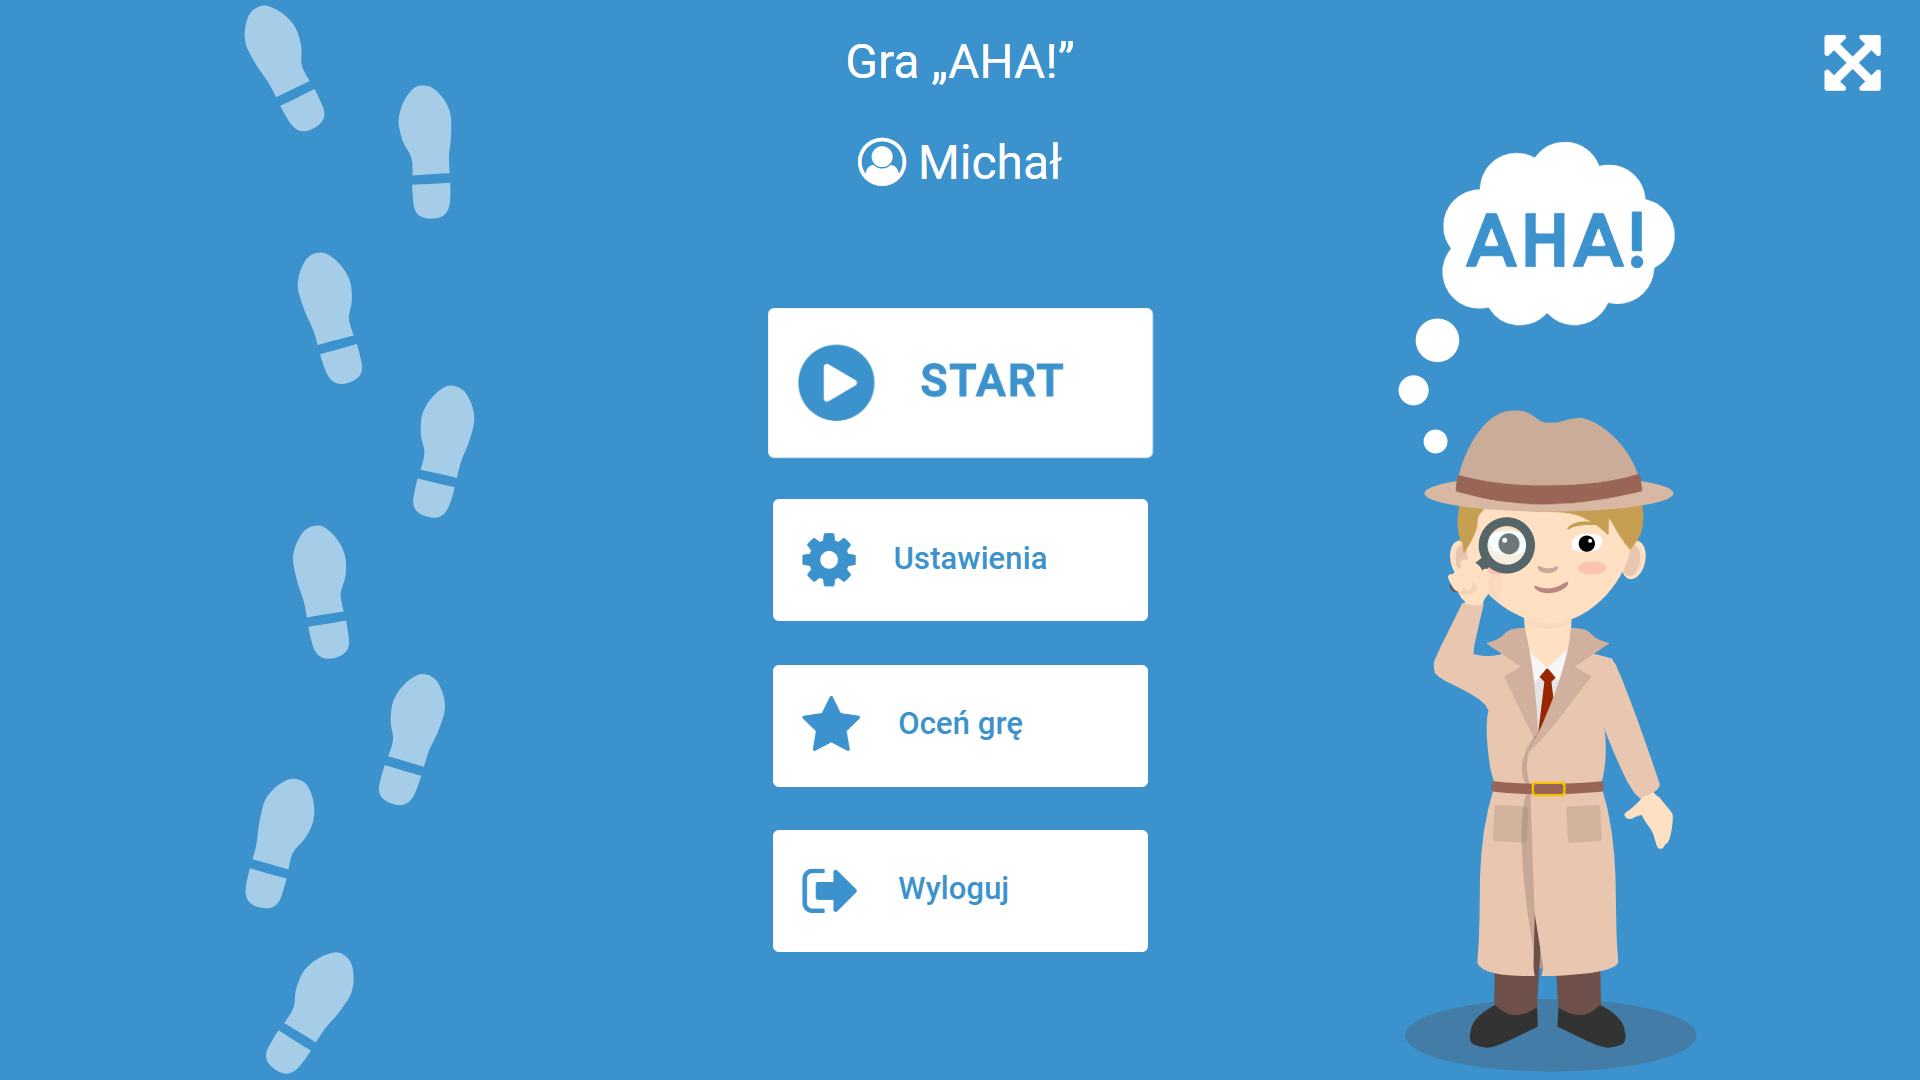
\includegraphics[width=\linewidth]{panel_gracza_01}
                \caption{}
            \end{subfigure}\hfill
            \begin{subfigure}{0.48\linewidth}
                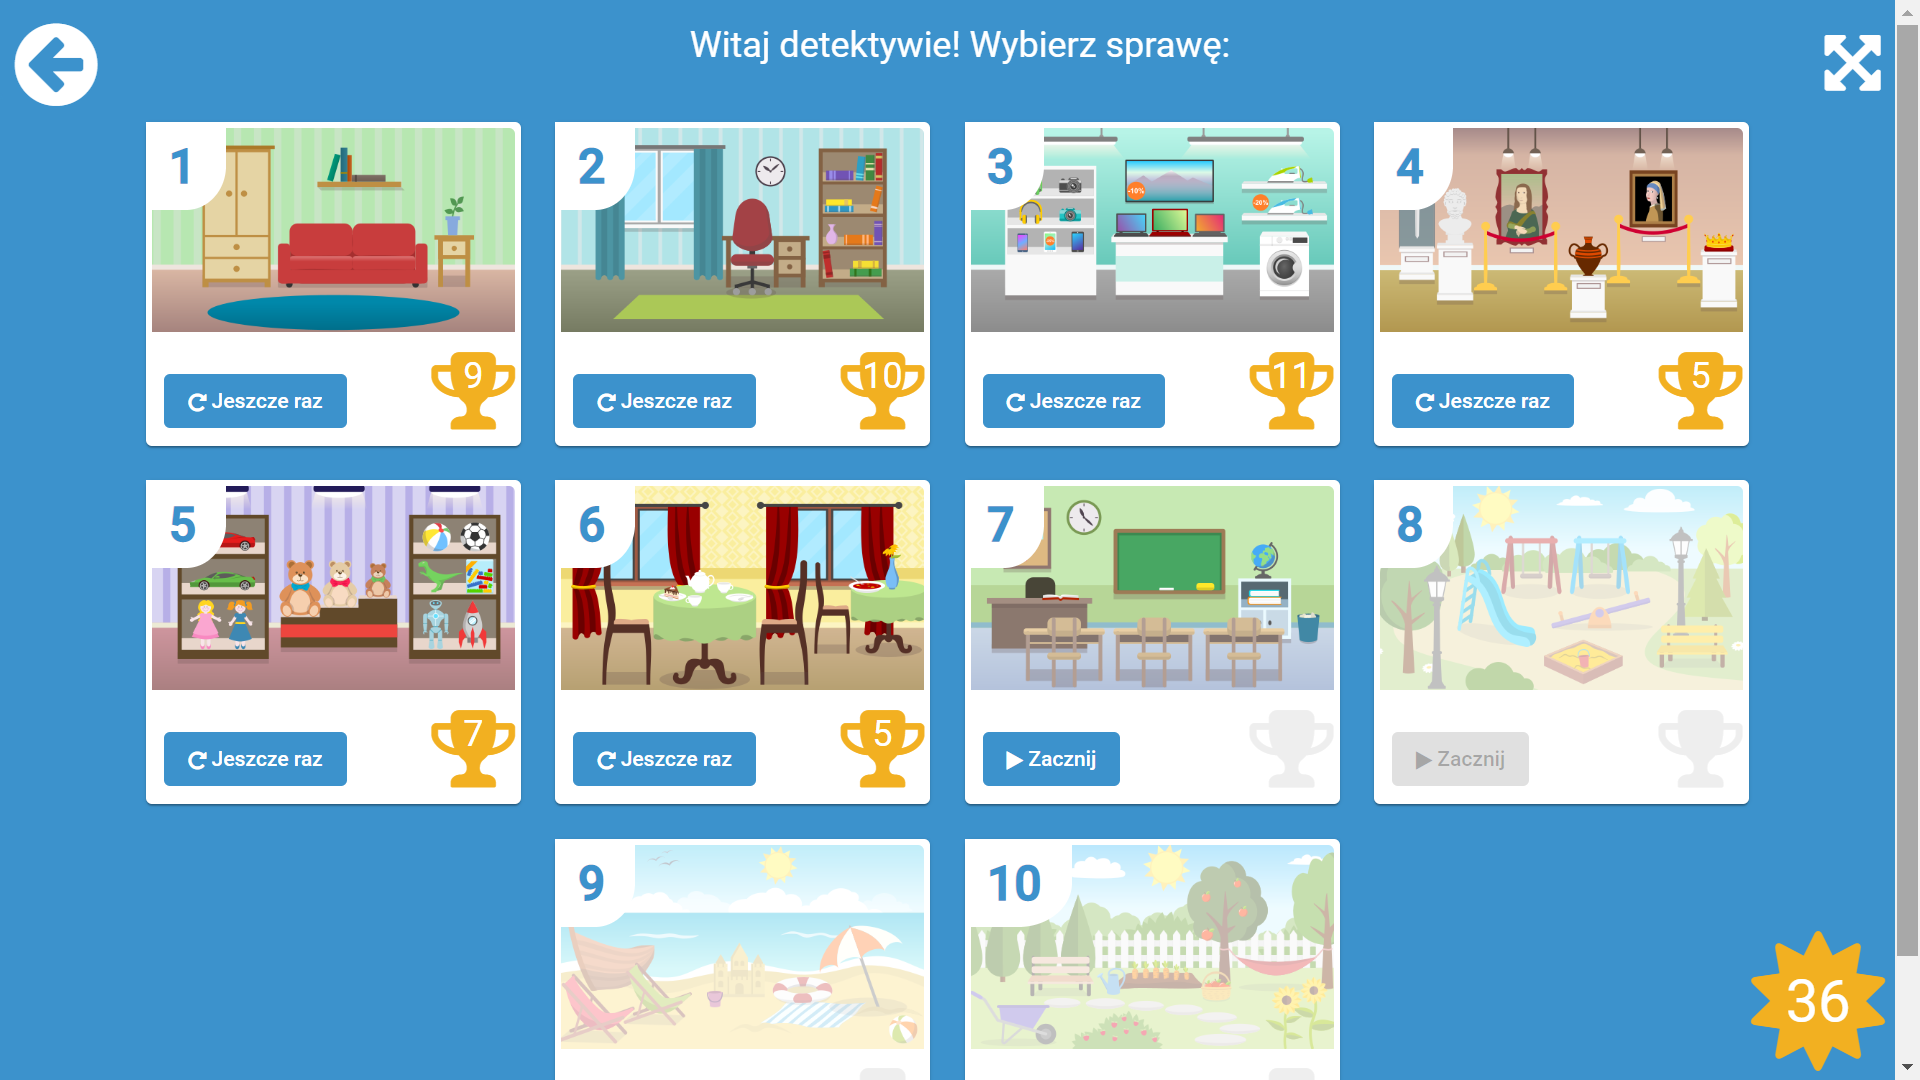
\includegraphics[width=\linewidth]{panel_gracza_02}
                \caption{}
            \end{subfigure}
            \par\bigskip
            \begin{subfigure}{0.48\linewidth}
                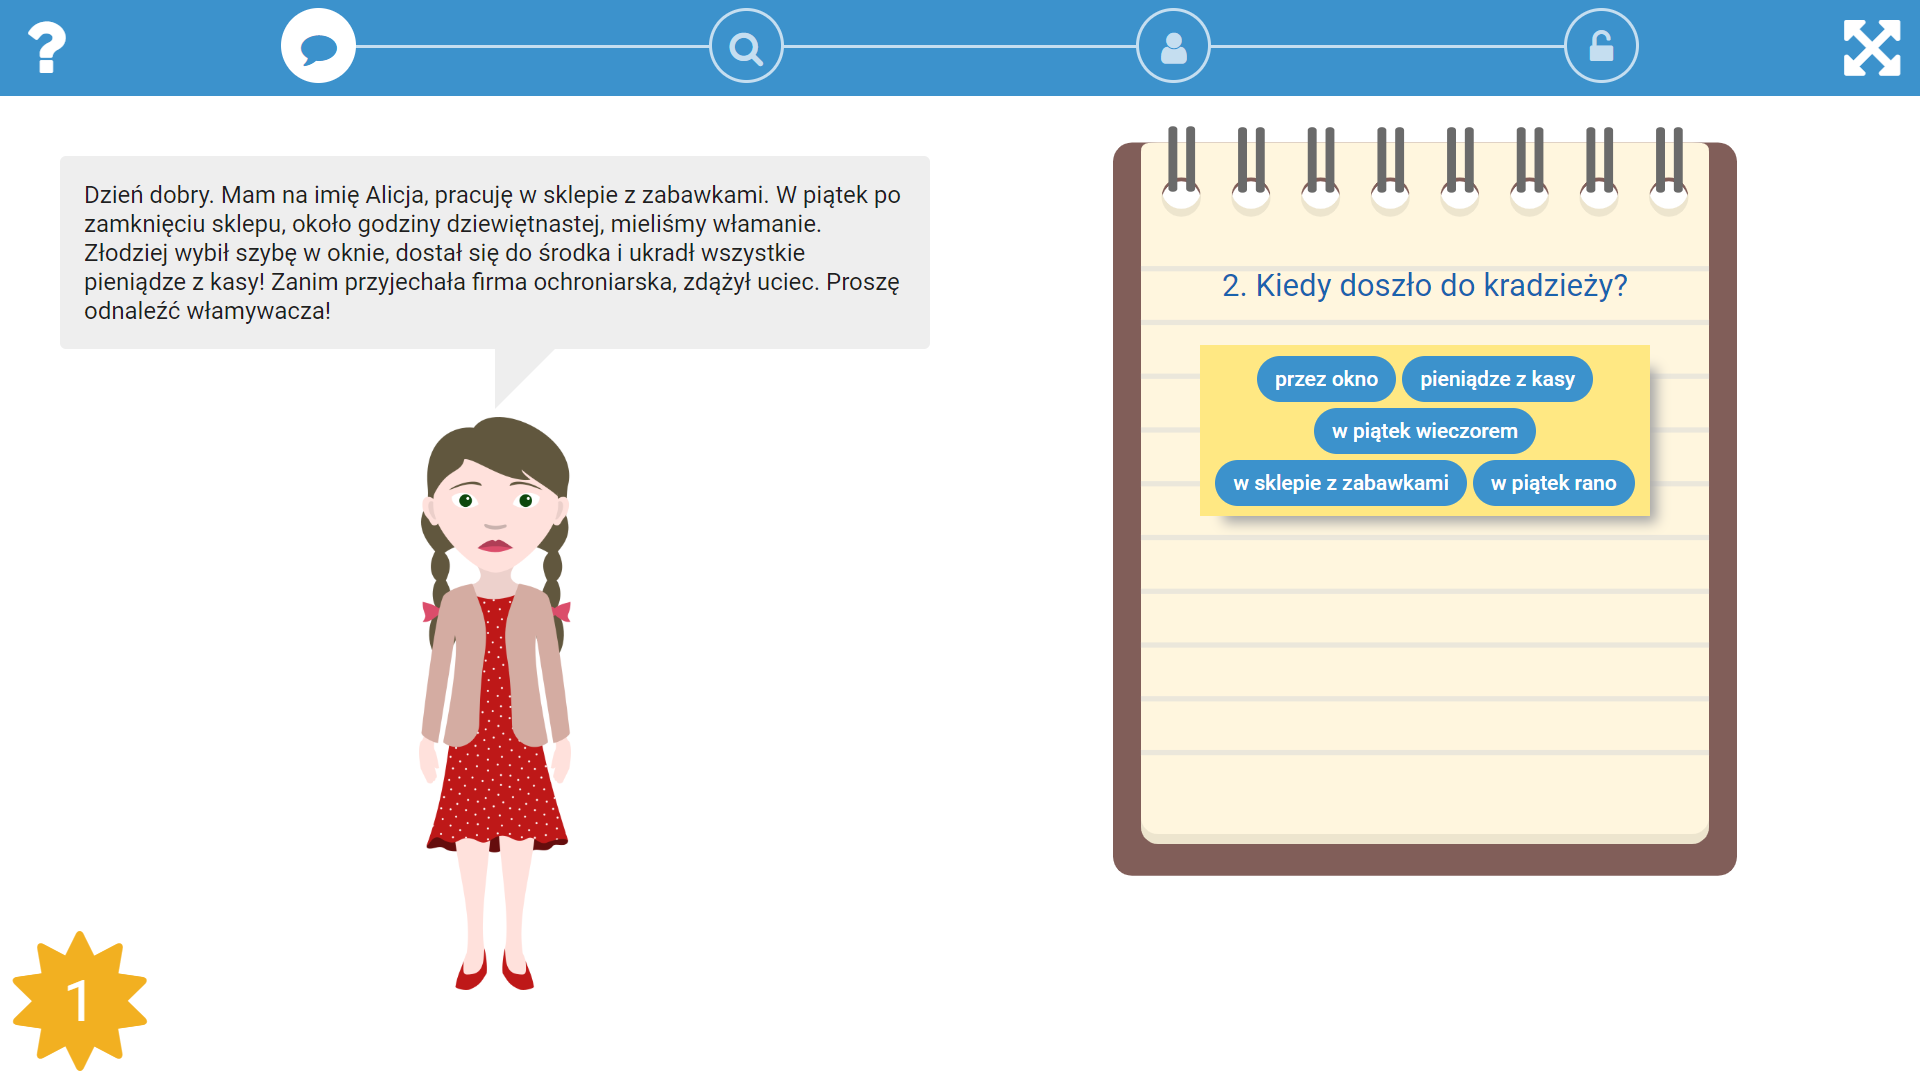
\includegraphics[width=\linewidth]{panel_gracza_03}
                \caption{}
            \end{subfigure}\hfill
            \begin{subfigure}{0.48\linewidth}
                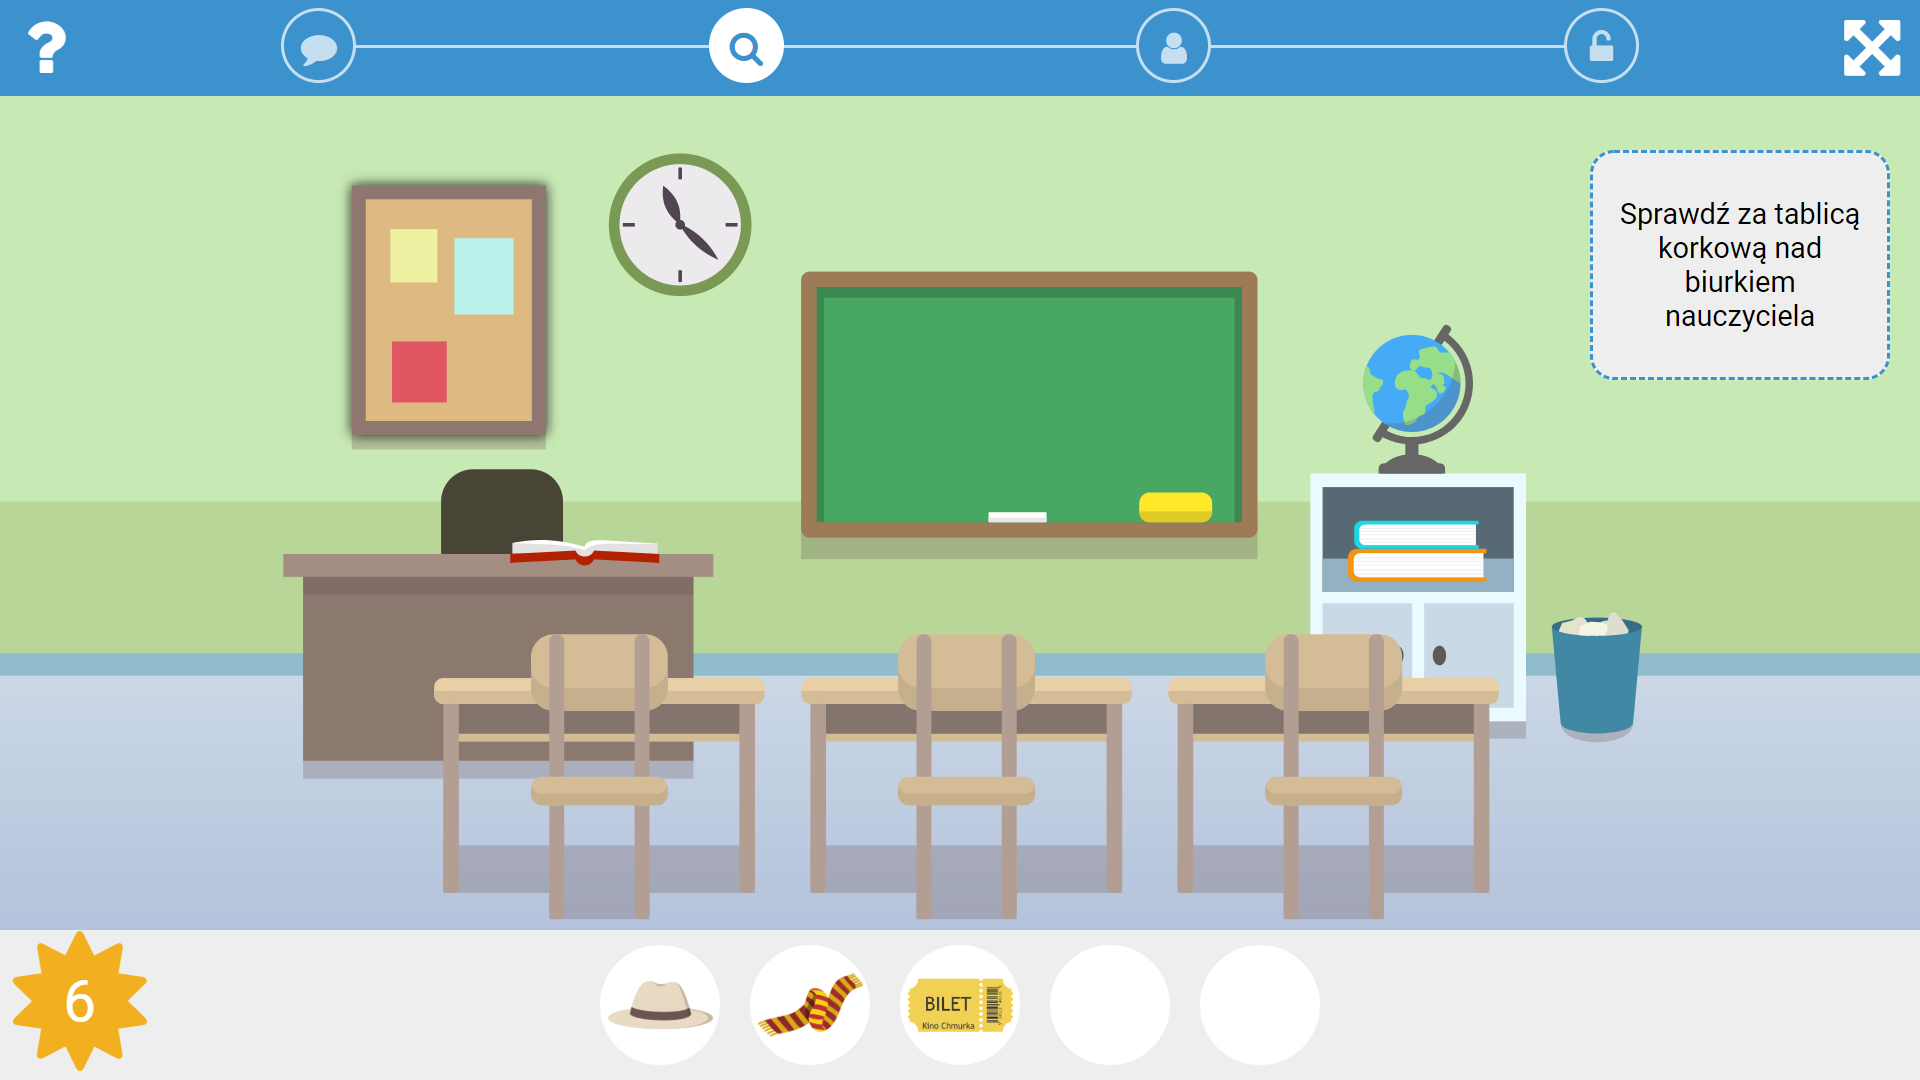
\includegraphics[width=\linewidth]{panel_gracza_04}
                \caption{}
            \end{subfigure}
            \par\bigskip
            \begin{subfigure}{0.48\linewidth}
                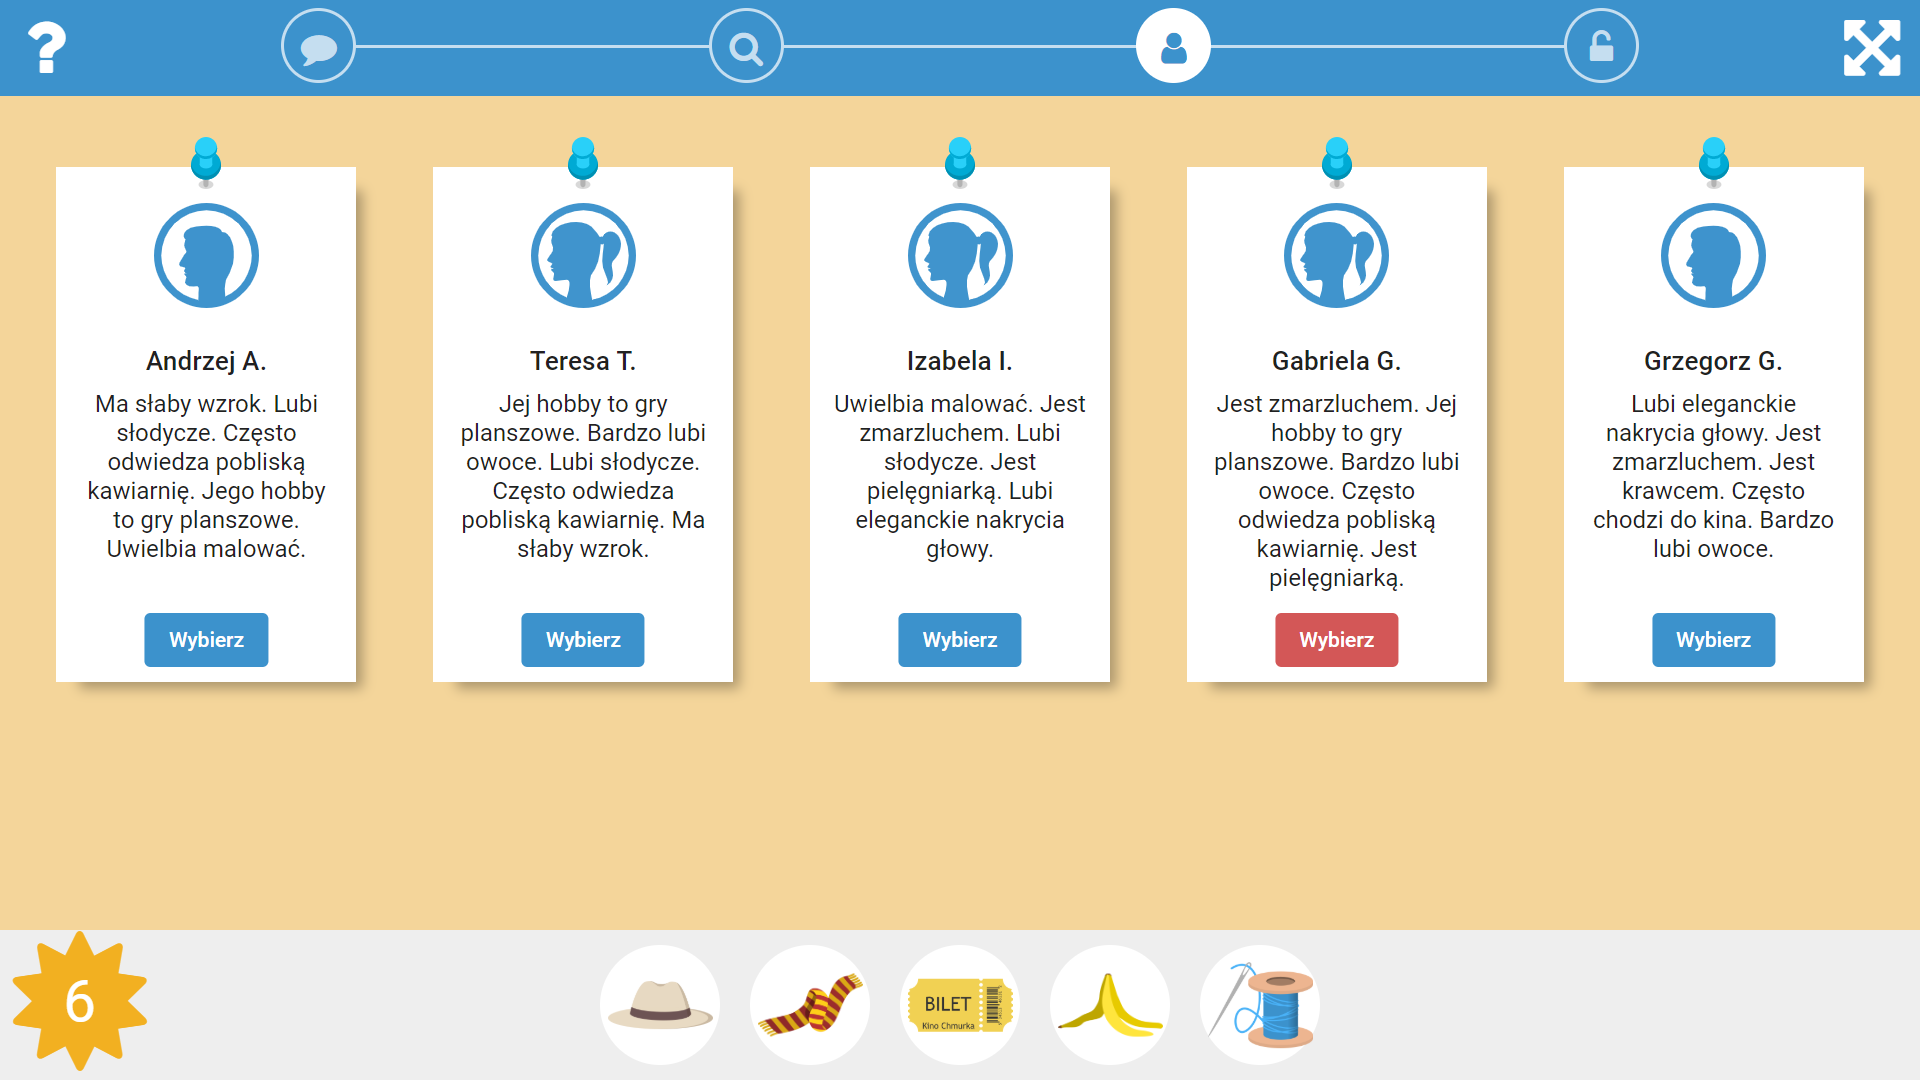
\includegraphics[width=\linewidth]{panel_gracza_05}
                \caption{}
            \end{subfigure}\hfill
            \begin{subfigure}{0.48\linewidth}
                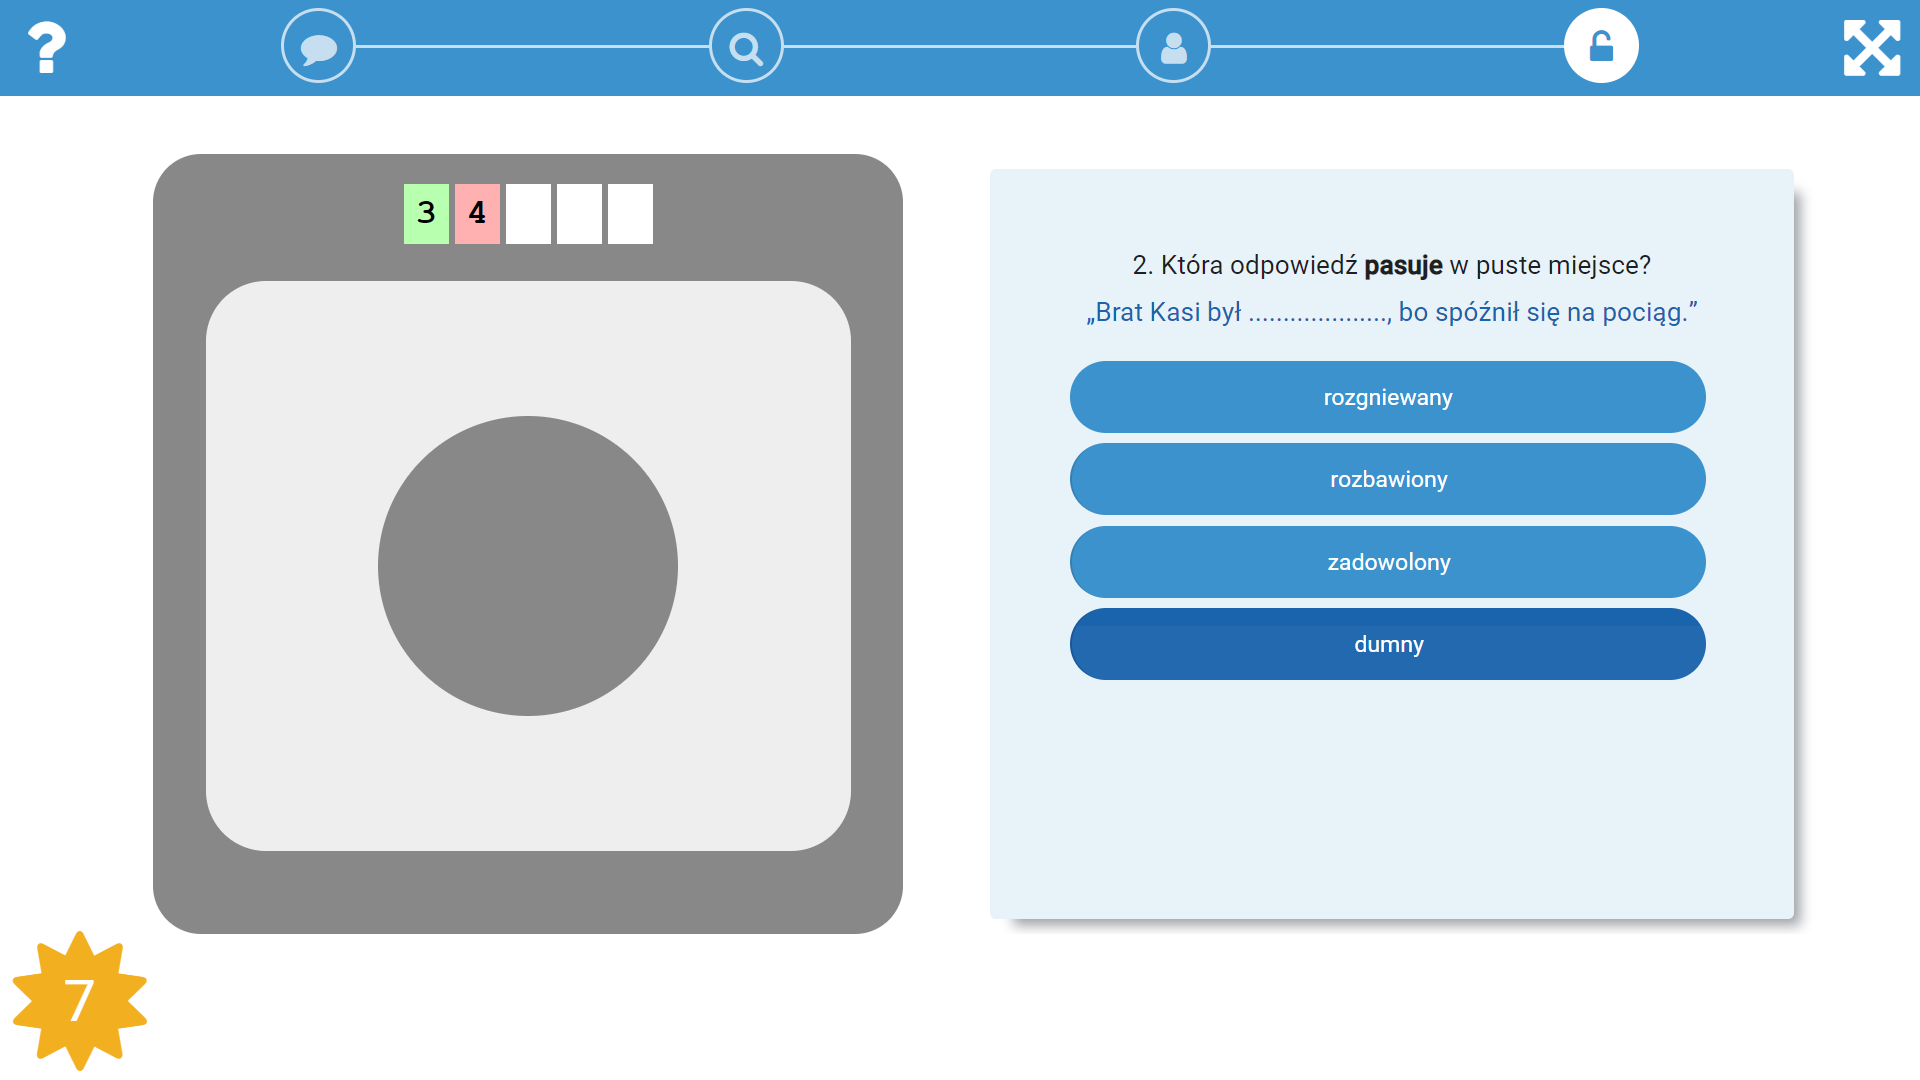
\includegraphics[width=\linewidth]{panel_gracza_06}
                \caption{}
            \end{subfigure}
            \par\bigskip
            \caption[Widok panelu gracza]
            {Widok panelu gracza \par \small (a) Menu gry. (b) Lista spraw. (c) Pierwsze zadanie (d) Drugie zadanie. (e) Trzecie zadanie. (f) Czwarte zadanie.}
            \label{fig:panelgracza}
        \end{figure}
        
        
    \subsection{Panel kontrolny}
        Użytkownik zarejestrowany jako opiekun może przeglądać statystyki gry oraz edytować treść gry graczy, którzy w ustawieniach swojego konta podali jego login (rys. \ref{fig:panelkontrolny}).
        
        Po zalogowaniu opiekun ma dostęp do listy graczy, zawierającej podstawowe informacje dotyczące każdego gracza (login gracza, datę ostatniej aktywności, liczbę ukończonych spraw, sumę najlepszych wyników) oraz opcje podglądu statystyk i edycji treści gry.
        Użytkownik może wyeksportować zbiorcze dane graczy do formatu arkusza kalkulacyjnego Microsoft Excel.
        
        \subsubsection{Podgląd statystyk gry}
        Po wybraniu opcji podglądu statystyk gracza użytkownik wskazuje jedną z dostępnych form wizualizacji (tabela, wykres punktowy lub wykres liniowy).
        W przypadku wyboru pierwszej wizualizacji wyświetlona zostaje tabela z wynikami wszystkich zadań.
        Dla każdego zadania podana jest data jego wykonania, numer sprawy, numer zadania, uzyskana liczba punktów, maksymalna liczba punktów oraz poprawność (iloraz uzyskanej i maksymalnej liczby punktów).
        Dane mogą być sortowane według każdego z atrybutów (domyślnie sortowanie następuje po dacie, malejąco).
        W przypadku wyboru wizualizacji w formie wykresu dane prezentowane są oddzielnie dla każdej sprawy.
        Pozioma oś stanowi oś czasu, pionowa przedstawia poprawność wykonania zadania (iloraz uzyskanej i maksymalnej liczby punktów).
        Na wykresie przedstawione są oznaczone kolorami wyniki dla każdego z czterech zadań.
        Klikając na elementy legendy użytkownik może wyłączać i włączać widoczność wyników poszczególnych zadań.
        
        \subsubsection{Edycja treści gry}
        W ramach opcji edycji treści gry danego gracza możliwa jest modyfikacja treści poszczególnych spraw oraz treści wspólnej dla wszystkich spraw. Jeśli treść danej sprawy lub treść wspólna była modyfikowana, poniżej formularza wyświetlona jest data ostatniej modyfikacji.
        Użytkownik ma również możliwość zresetowania treści poszczególnej sprawy oraz treści wspólnej do ustawień domyślnych.

        Aby modyfikować treść danej sprawy użytkownik wybiera ją z listy zawierającej ilustracje miejsc przestępstwa występujące w poszczególnych sprawach.
        Następnie za pomocą formularza edycji może modyfikować warianty szczegółów sprawy -- dodać, edytować lub usunąć wariant (jeśli liczba wariantów jest większa niż jeden).
        Modyfikacja wariantu obejmuje wybór ilustracji skradzionego przedmiotu i postaci, edycję wypowiedzi postaci oraz pytań wraz z odpowiedziami, w tym dodawanie nowych i usuwanie (jeśli liczba pytań jest większa niż dwa).
        Użytkownik może również usuwać wybrane instrukcje przeszukiwania (jeśli liczba instrukcji jest większa niż cztery), a także edytować liczbę śladów do odnalezienia (w przedziale od trzech do sześciu) oraz liczbę pytań jednokrotnego wyboru poszczególnych typów (w przedziale od zera do siedmiu, przy sumarycznej liczbie pytań wynoszącej minimum dwa ).
        Jeśli formularz edycji nie zawiera błędów użytkownik może zapisać zmiany.
        
        Formularz edycji treści wspólnej dla wszystkich spraw pozwala na modyfikację opisów podejrzanych oraz zadań jednokrotnego wyboru.
        Użytkownik może edytować zdania opisujące cechy podejrzanych oraz usuwać wybrane przykłady, jeśli liczba zdań w danej kategorii (zdanie opisujące zawód lub inną cechę) wynosi więcej niż sześć.
        W ramach edycji zadań jednokrotnego wyboru istnieje możliwość edytowania, dodawania lub usuwania kategorii semantycznych oraz zdań z luką.
        Minimalna liczba kategorii semantycznych oraz zdań z luką wynosi siedem.
        Minimalna liczba słów w kategorii semantycznej oraz pasujących i niepasujących odpowiedzi dla zdań z luką wynosi cztery.
        
        \begin{figure}
            \centering
            \begin{subfigure}{0.48\linewidth}
                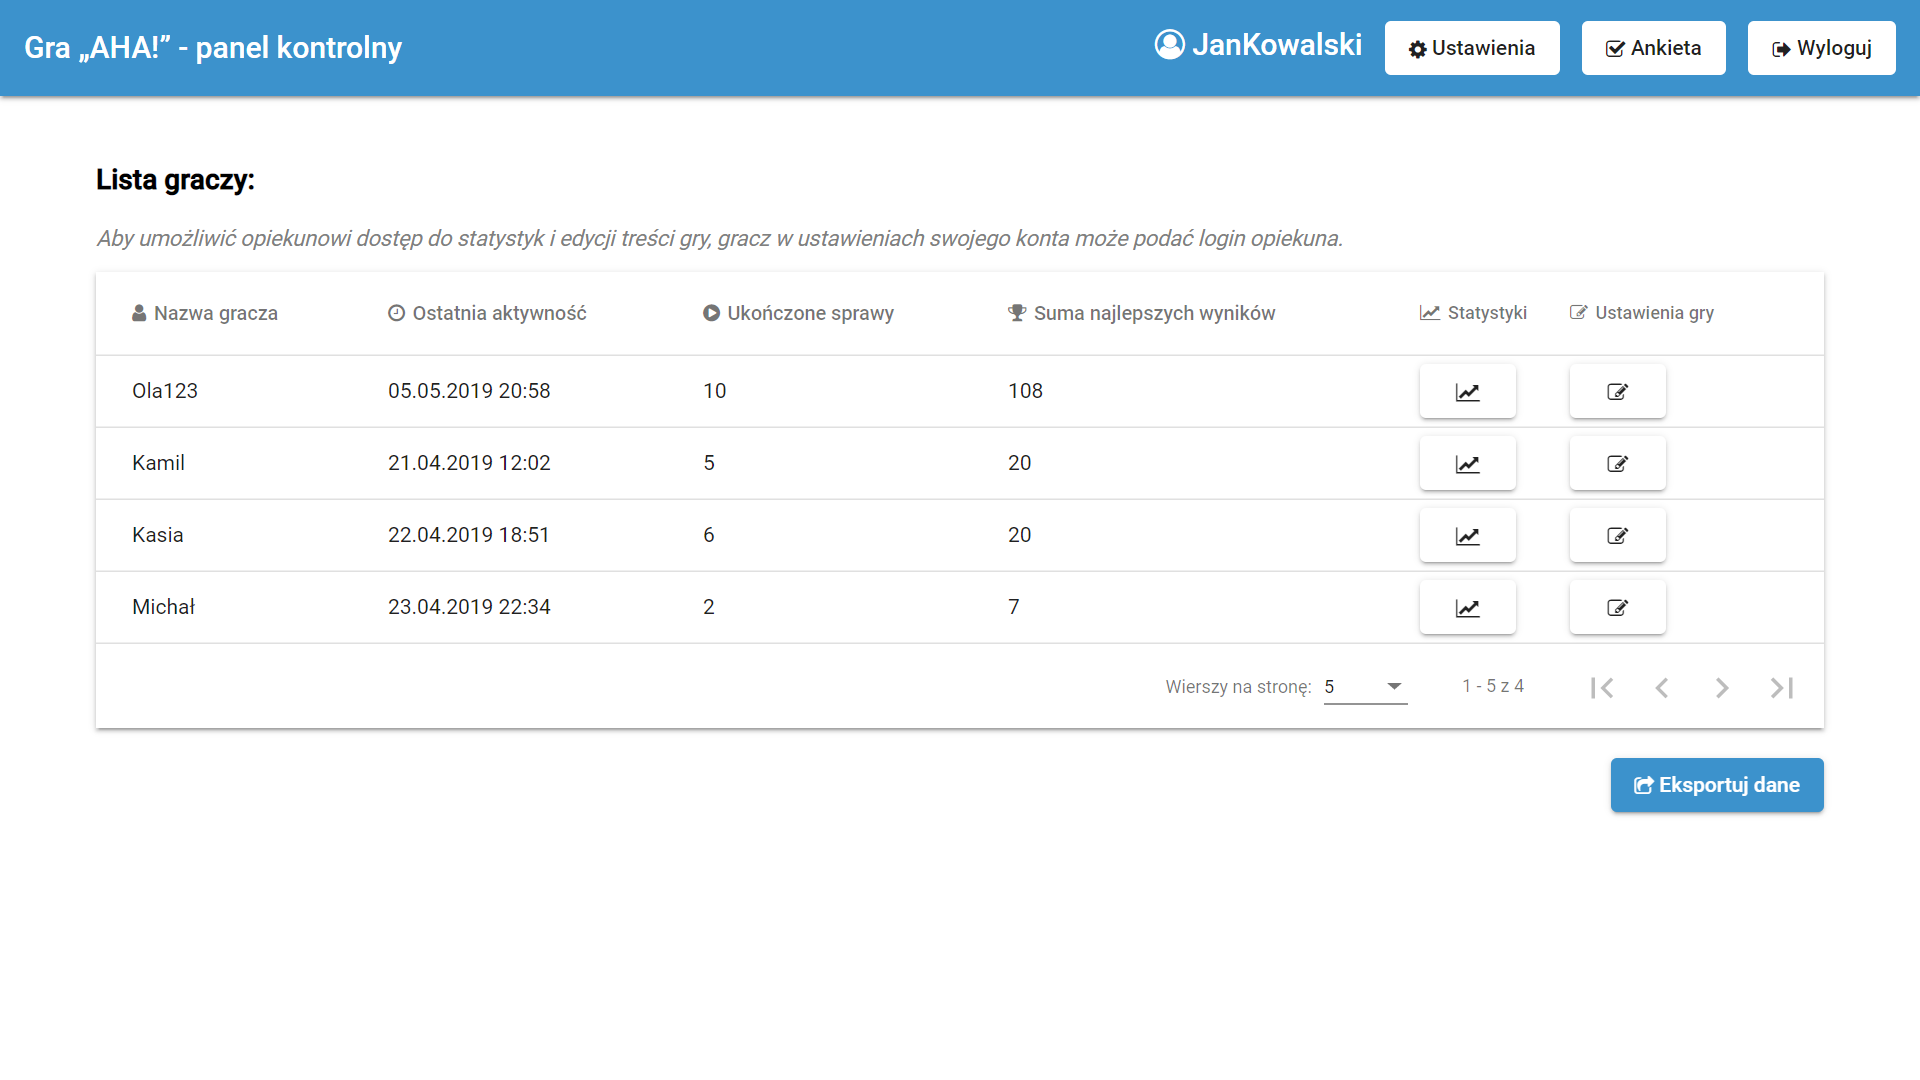
\includegraphics[width=\linewidth]{panel_kontrolny_01}
                \caption{}
            \end{subfigure}\hfill
            \begin{subfigure}{0.48\linewidth}
                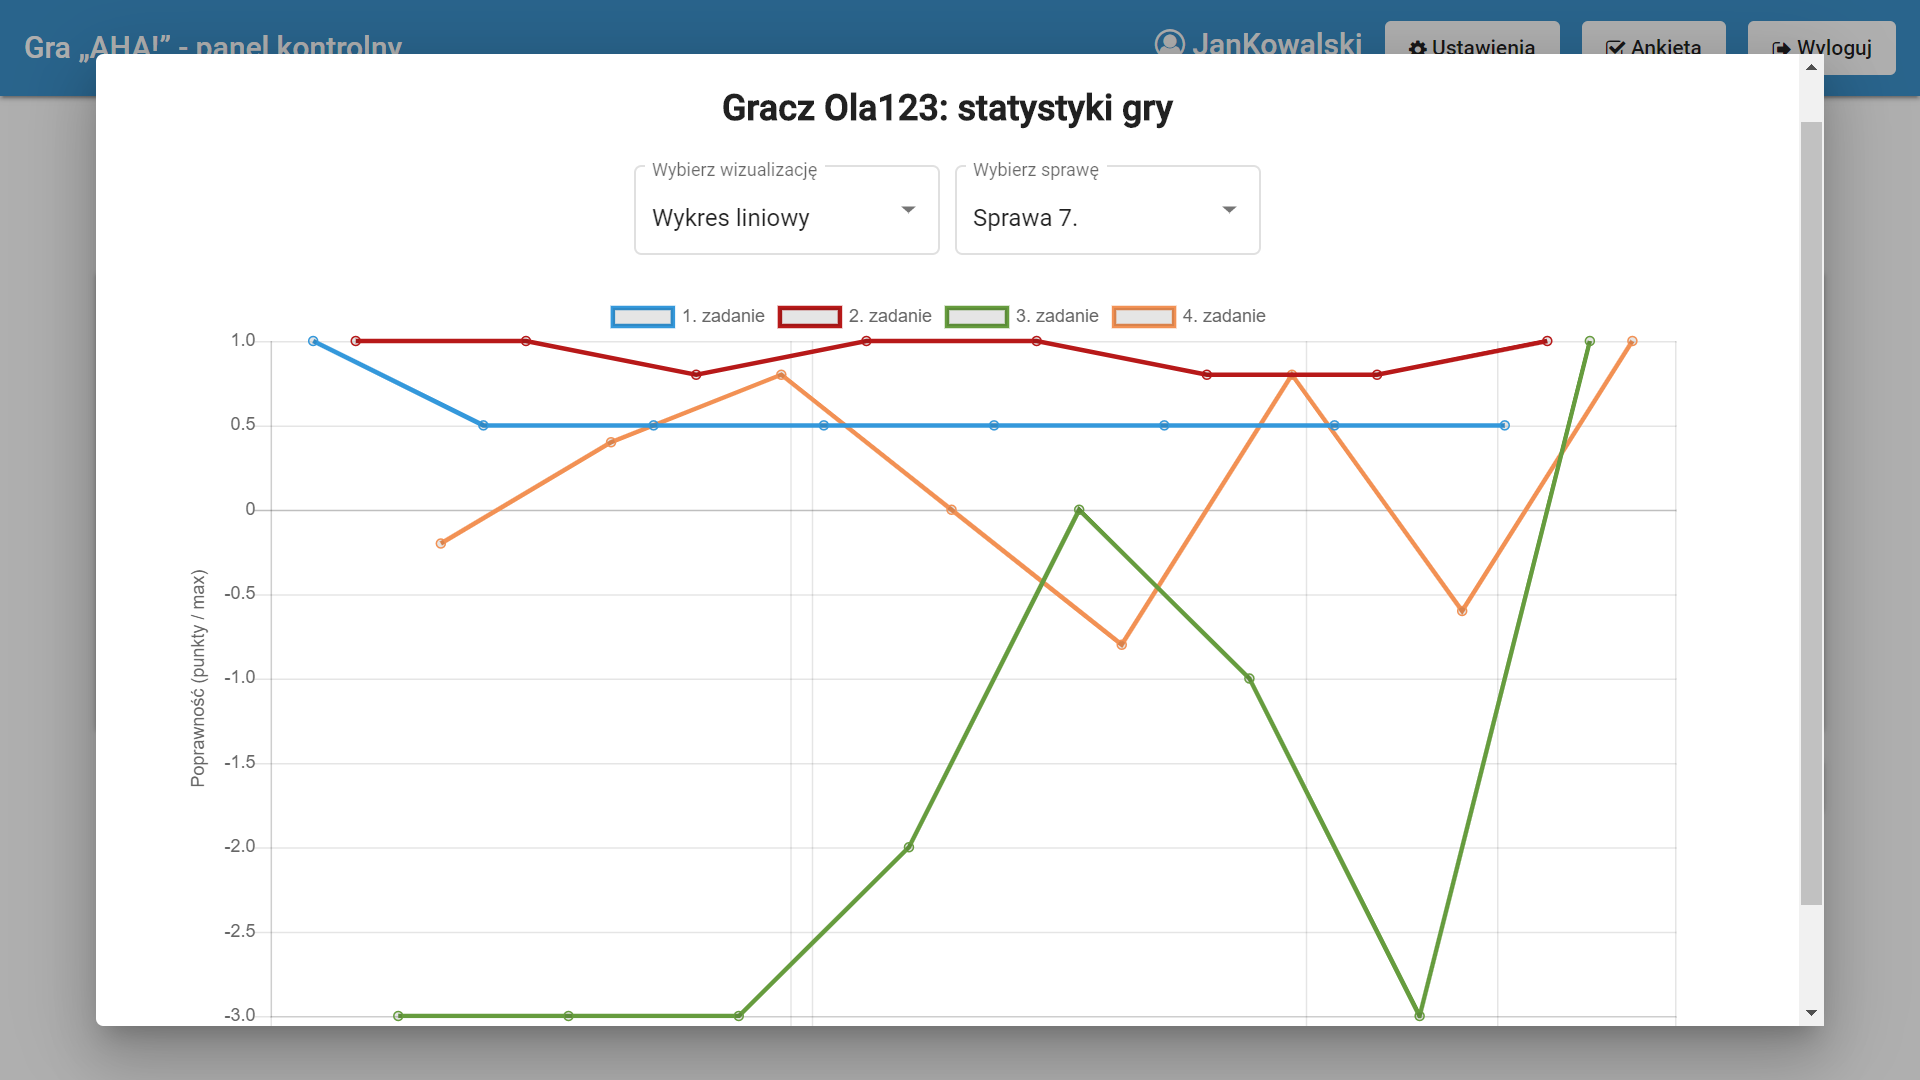
\includegraphics[width=\linewidth]{panel_kontrolny_02}
                \caption{}
            \end{subfigure}
            \par\bigskip
            \begin{subfigure}{0.48\linewidth}
                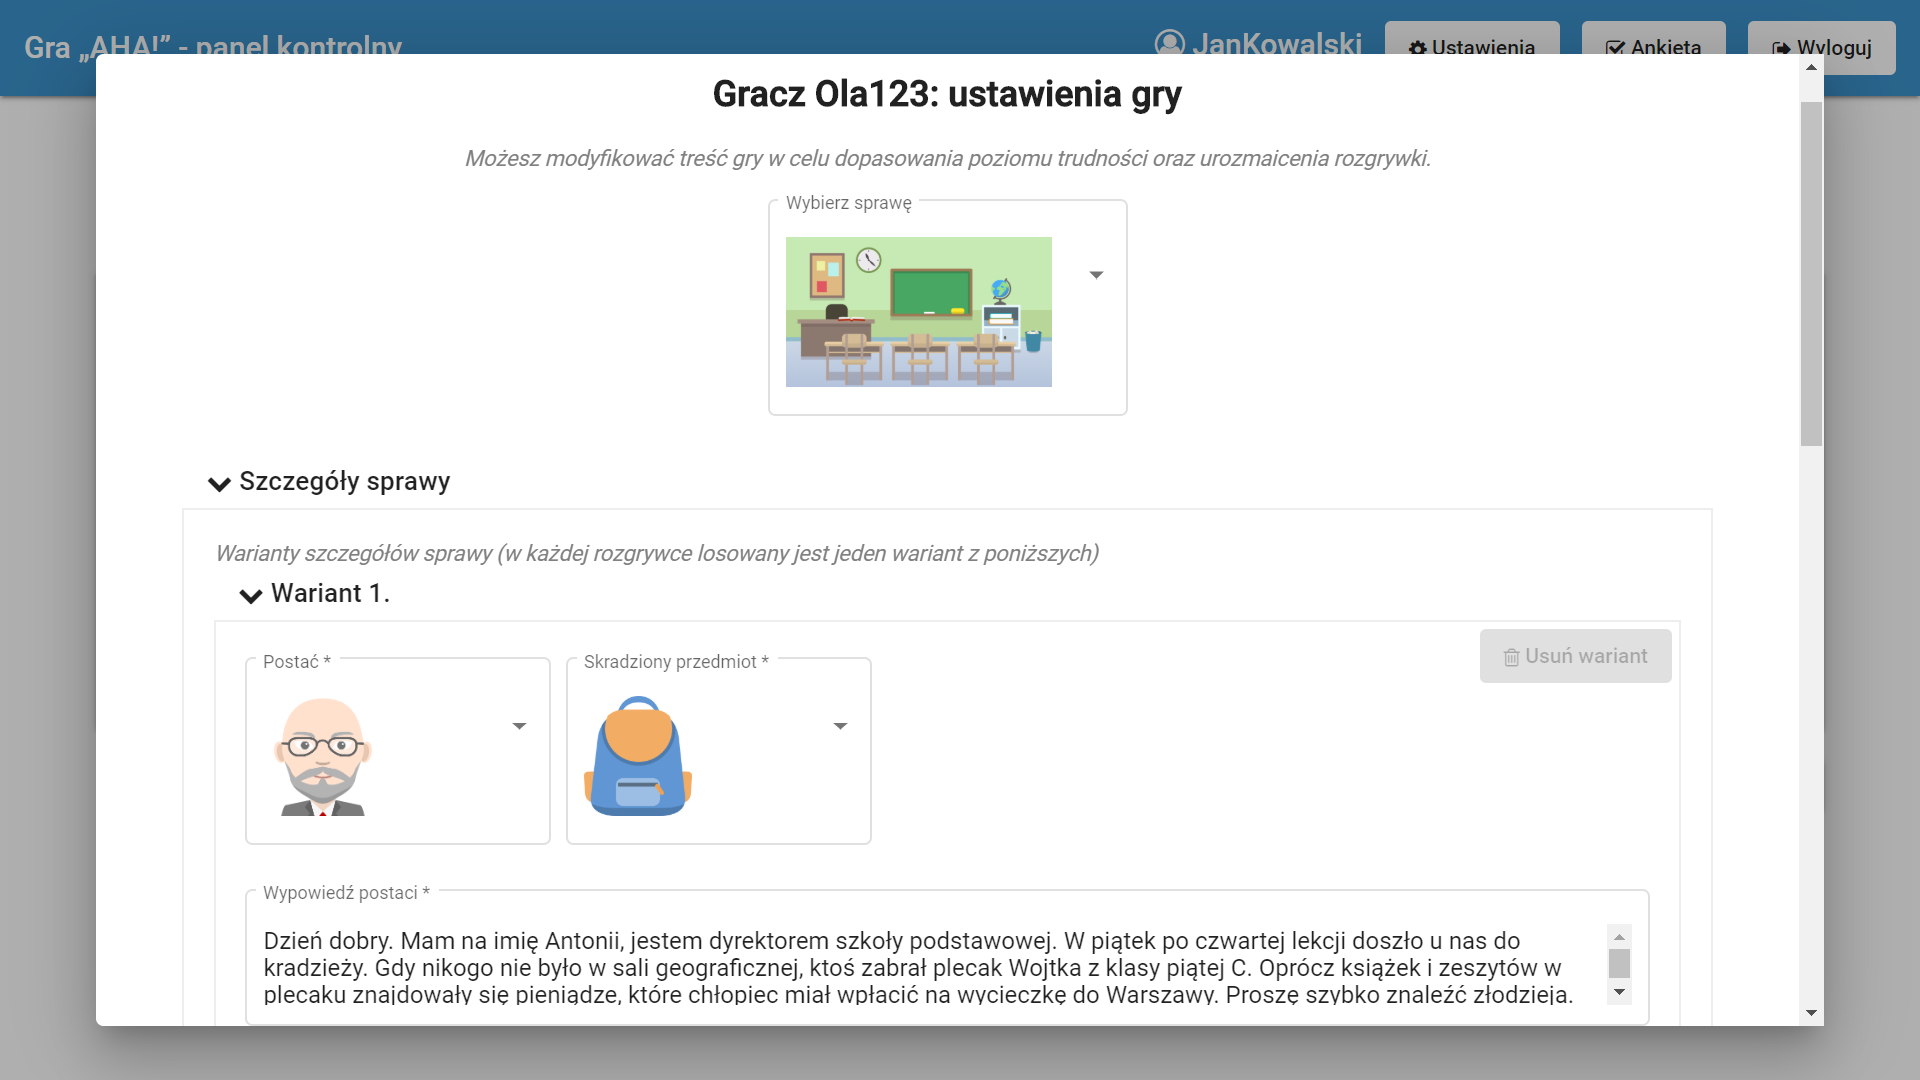
\includegraphics[width=\linewidth]{panel_kontrolny_03}
                \caption{}
            \end{subfigure}\hfill
            \begin{subfigure}{0.48\linewidth}
                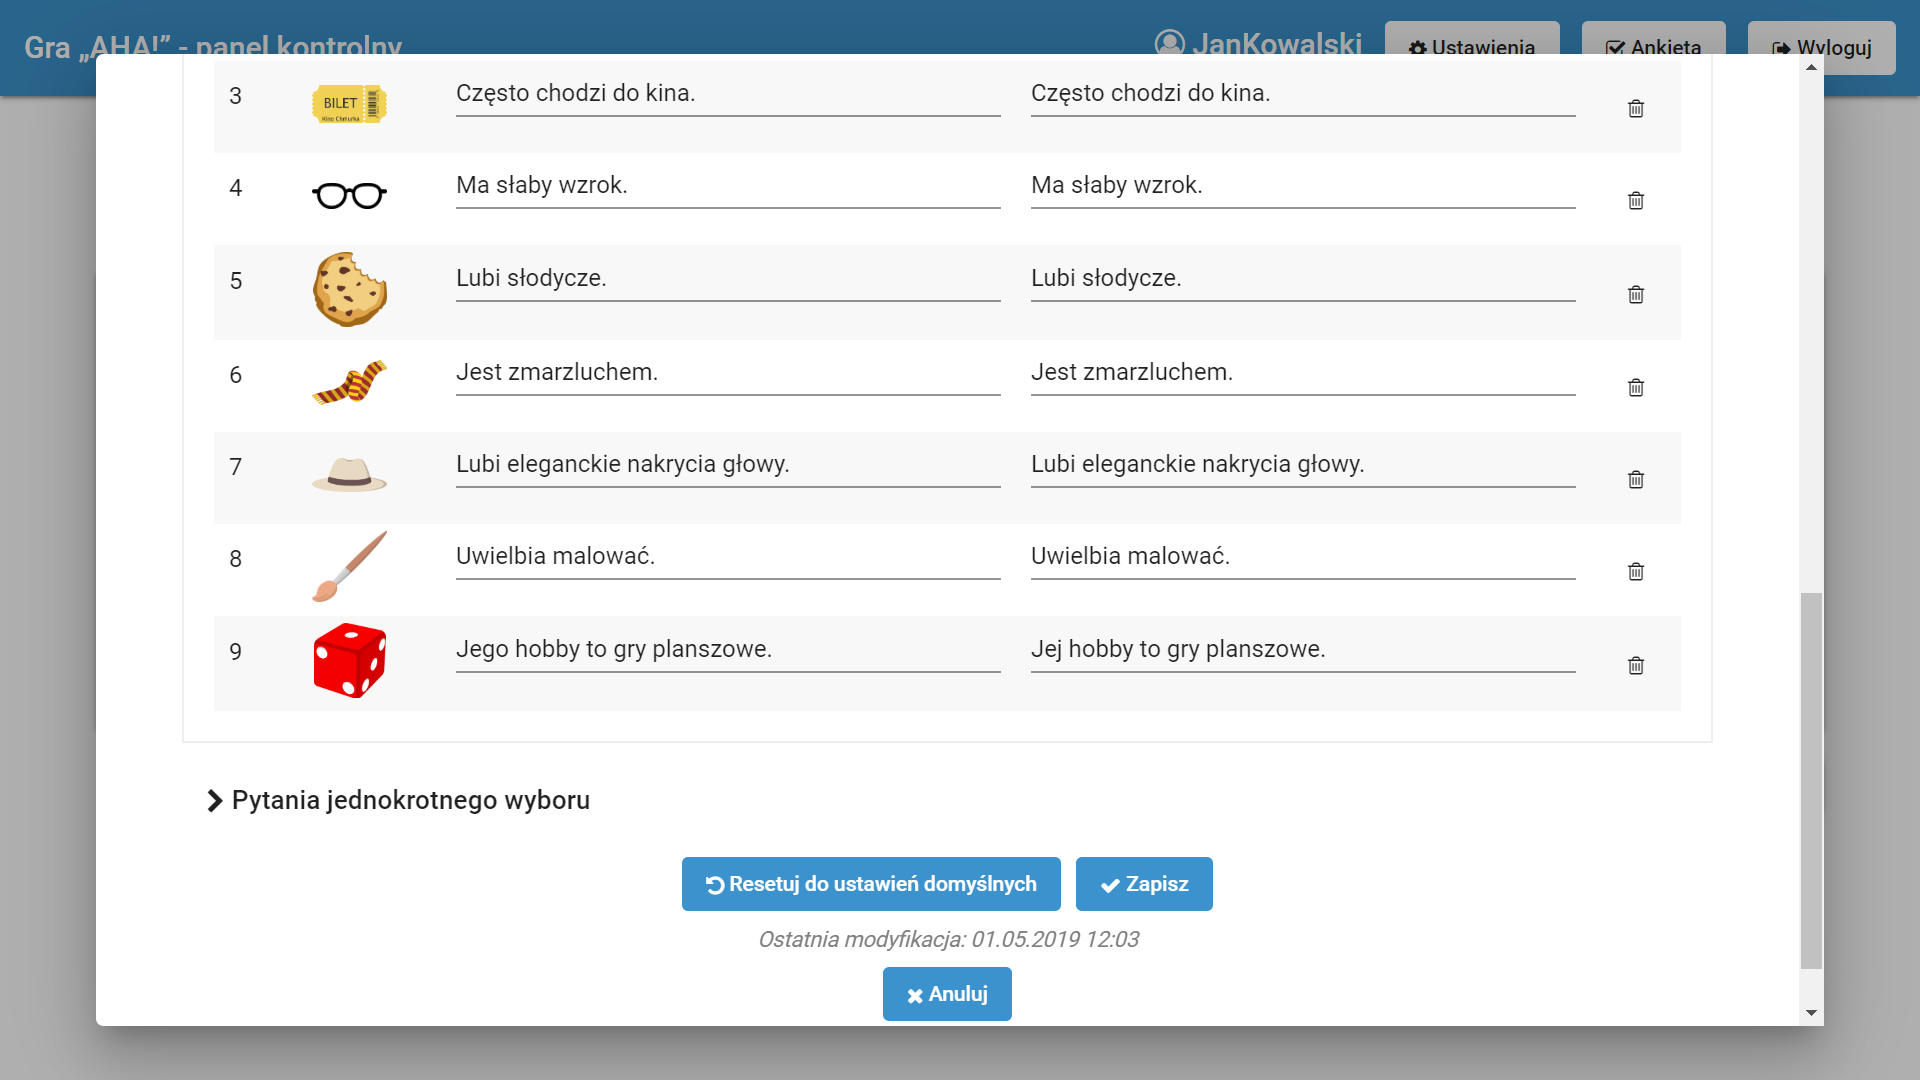
\includegraphics[width=\linewidth]{panel_kontrolny_04}
                \caption{}
            \end{subfigure}
            \par\bigskip
            \caption[Widok panelu kontrolnego]
            {Widok panelu kontrolnego \par \small (a) Lista graczy. (b) Podgląd statystyk gry. (c), (d) Edycja treści gry.}
            \label{fig:panelkontrolny}
        \end{figure}

    \subsection{Ankiety}
        Po zalogowaniu użytkownik ma możliwość wypełnienia krótkiej ankiety oceniającej atrakcyjność wizualną i tematyczną, łatwość użycia oraz przydatność gry (tab. \ref{table:ankieta}).
        Ankieta w wersji dla opiekuna (dostępna z poziomu panelu kontrolnego) zawiera siedem pytań z pięciostopniową skalą Likerta (,,nie'', ,,raczej nie'', ,,nie mam zdania'', ,,raczej tak'', ,,tak'').
        Ankieta w wersji dla gracza (dostępna w menu gry), składa się z pięciu pytań z uproszczoną, trzystopniową skalą odpowiedzi (,,nie'', ,,nie wiem'', ,,tak'').
        Obie wersje ankiety zawierają również pole tekstowe na opcjonalne uwagi.
        Po wysłaniu ankieta zapisywana jest w bazie danych.

        \begin{table}
            \begin{tabularx}{\textwidth}{ l X }
             \hline
             
             \hline
                & \textbf{Pytania w wersji dla opiekuna} \\
             \hline
             1. & Czy tematyka gry jest ciekawa? \\
             2. & Czy gra jest atrakcyjna wizualnie? \\
             3. & Czy gra jest łatwa w użytkowaniu? \\
             4. & Czy panel kontrolny jest prosty w obsłudze? \\
             5. & Czy trudność zadań jest odpowiednia? \\
             6. & Czy gra jest użyteczna w ćwiczeniu czytania ze zrozumieniem? \\
             7. & Czy poleciłby/aby Pan/i tę grę jako pomoc edukacyjną? \\
             \hline
             
             \hline
                & \textbf{Pytania w wersji dla gracza} \\
             \hline
                1. & Czy lubisz grać w tę grę? \\
                2. & Czy gra jest ciekawa? \\
                3. & Czy podoba Ci się grafika? \\
                4. & Czy gra jest prosta w użyciu? \\
                5. & Czy poleciłbyś/poleciłabyś tę grę kolegom i koleżankom? \\
             \hline
             
             \hline
            \end{tabularx}
            \caption{Pytania zawarte w ankiecie}
            \label{table:ankieta}
        \end{table}


% \section{Struktura aplikacji} // w załączniku?
% diagram UML